% Ozimut - the Ozimut method: the white paper (English translation of methode-ozimut.tex, 2026-10-17; keep the two in step).
% Build: py -3 docs/whitepaper/build.py (figures and numbers, French and English, pdflatex x2 each; this PDF moved to
% site/assets/ozimut-methode.en.pdf and copied to ocn-methode-top.en.pdf, its former name). Figures from fig/en/, numbers
% from numbers.en.tex (figures.py --lang en). Aggregate figures only: no name, no personal result. Vocabulary:
% docs/i18n/glossary.md. 2026-10-19 (owner): the site O'CN renamed Ozimut, the "Top" method the Ozimut method (Ozimut
% index, Ozimut score, course's Ozimut value); the geometric pair no longer a method: one line among the variants set
% aside. Formerly methode-top.en.tex.
\documentclass[11pt,a4paper]{article}
\usepackage[utf8]{inputenc}
\usepackage[T1]{fontenc}
\usepackage{lmodern}
\usepackage[british]{babel}
\usepackage[margin=24mm]{geometry}
\usepackage{amsmath}
\usepackage{booktabs}
\usepackage{graphicx}
\usepackage{microtype}
\usepackage{xcolor}
\usepackage[colorlinks=true,linkcolor=black,urlcolor=blue!50!black,citecolor=black]{hyperref}
\usepackage{caption}
\captionsetup{font=small,labelfont=bf}
\setlength{\parskip}{4pt}
\graphicspath{{fig/en/}}
\newcommand{\CN}{\textsc{cn}}
% generated by figures.py --lang en: the numbers the English text quotes (2026-10-19)
\newcommand{\NaccFoff}{79.31}
\newcommand{\NaccFtop}{81.61}
\newcommand{\NrrFoff}{53.9}
\newcommand{\NrrFtop}{64.8}
\newcommand{\NgainF}{$+$2.31 [$+$2.19, $+$2.43]}
\newcommand{\NgainRF}{$+$10.8 [$+$10.2, $+$11.5]}
\newcommand{\NcompsF}{1,941}
\newcommand{\NaccSoff}{81.42}
\newcommand{\NaccStop}{83.70}
\newcommand{\NrrSoff}{63.2}
\newcommand{\NrrStop}{68.0}
\newcommand{\NgainS}{$+$2.28 [$+$1.96, $+$2.58]}
\newcommand{\NgainRS}{$+$4.8 [$+$1.6, $+$7.1]}
\newcommand{\NcompsS}{588}
\newcommand{\NgainNF}{$+$1.23 [$+$1.05, $+$1.39]}
\newcommand{\NgainNS}{$+$1.35 [$+$0.22, $+$2.40]}
\newcommand{\NwinsF}{15 of 15}
\newcommand{\NwinsS}{11 of 15}
\newcommand{\NnineVsAll}{$+$0.08 [$+$0.06, $+$0.10]}
\newcommand{\NnineVsAllN}{$+$0.12 [$+$0.08, $+$0.16]}
\newcommand{\NnineBetter}{8}
\newcommand{\NnineWorse}{1}
\newcommand{\NallVsTwoF}{$+$0.34 [$+$0.29, $+$0.39]}
\newcommand{\NallVsTwoS}{$-$0.34 [$-$0.42, $-$0.27]}
\newcommand{\NvttEightyFive}{$+$0.20 [$+$0.11, $+$0.29]}
\newcommand{\NvttEightyFiveT}{$-$0.49 [$-$0.88, $-$0.13]}
\newcommand{\NvttSeventyFive}{$+$0.15 [$+$0.09, $+$0.20]}
\newcommand{\NeligFifty}{$-$0.03 [$-$0.04, $-$0.02]}
\newcommand{\NeligSeventy}{$-$0.11 [$-$0.13, $-$0.09]}
\newcommand{\NeligAll}{$-$0.62 [$-$0.68, $-$0.57]}
\newcommand{\NoneCn}{$-$0.10 [$-$0.11, $-$0.08]}
\newcommand{\NoneCnT}{$-$0.38 [$-$0.44, $-$0.31]}
\newcommand{\NmleS}{$+$0.37}
\newcommand{\NmleF}{$-$1.62}
\newcommand{\NgeoVarF}{$-$0.02 [$-$0.03, $-$0.01]}
\newcommand{\NgeoVarS}{$+$0.15 [$+$0.10, $+$0.20]}
\newcommand{\NtruncF}{4.8}
\newcommand{\NtruncS}{2.8}
\newcommand{\NcalibYoungOff}{8.9}
\newcommand{\NjunF}{$+$0.18 [$+$0.16, $+$0.21]}
\newcommand{\NjunFT}{$+$0.14 [$+$0.08, $+$0.20]}
\newcommand{\NjunS}{$+$0.11 [$+$0.05, $+$0.17]}
\newcommand{\NjunST}{$+$0.04 [$-$0.07, $+$0.17]}
\newcommand{\NjunV}{$+$0.15 [$+$0.10, $+$0.19]}
\newcommand{\NjunVT}{$+$0.28 [$+$0.07, $+$0.53]}
\newcommand{\NjunFBetter}{15}
\newcommand{\NjunAdult}{$+$0.08 [$+$0.06, $+$0.10]}
\newcommand{\NjunBoth}{$+$0.16 [$+$0.14, $+$0.19]}
\newcommand{\NjunWin}{$-$0.59 [$-$0.63, $-$0.54]}
\newcommand{\NjunTop}{$-$0.08 [$-$0.10, $-$0.06]}
\newcommand{\NjunBiasBefore}{$+$2.3}
\newcommand{\NjunBiasAfter}{$+$3.9}
\newcommand{\NoutFast}{$-$0.21 [$-$0.25, $-$0.17]}
\newcommand{\NoutFastFive}{$-$1.06 [$-$1.12, $-$0.99]}
\newcommand{\NoutLoop}{25}
\newcommand{\NoutBothF}{$-$0.37 [$-$0.40, $-$0.34]}
\newcommand{\NoutXS}{$+$0.29 [$+$0.22, $+$0.35]}
\newcommand{\NoutXV}{$+$0.29 [$+$0.17, $+$0.40]}


\title{The Ozimut method\\\large The national ranking recalculated: aims, method, study and results}
\author{Ozimut — Orienteering, in maps and numbers\\\small \url{https://ozimut.com} — an independent site, not affiliated with FFCO}
\date{19 October 2026}

\begin{document}
\maketitle

\begin{abstract}
Starting from the same results as the French orienteering federation (Fédération française de course d'orientation, FFCO), the Ozimut site calculates an alternative national ranking, the Ozimut method, and compares it with the official ranking over fifteen seasons. The Ozimut method keeps FFCO's race score and ordinary means: anyone can work out a score or an index by hand. It changes only what matters: the best races kept, filling six places; a share of the field, set for each discipline, to measure how hard the courses are; a continuous rescaling; and juniors' races that count less and less as they age.

Over the 2012 to 2024 seasons, which were not used to tune the method, the Ozimut index picks the right winner in \NaccFtop\% of duels between two runners on the same course in forest, against \NaccFoff\% for the official \CN; in sprint, \NaccStop\% against \NaccSoff\%.
\end{abstract}

\tableofcontents

\section{Aims}

The national ranking (\CN) serves two different purposes. It is used to measure how hard courses are: for that, we need the usual level of the runners present, without a single bad run or a one-off exploit distorting it. It is also used to rank runners: for qualification to the French championships, we need to know what a runner can do in a major competition, and so to look at their best races.

The alternative method had to:
\begin{itemize}
  \item start from the same results and the same race score as FFCO, so that anyone can understand and check it;
  \item count the French championships and the national races, which the official method often leaves out;
  \item not penalise a runner for running one more race, once their best races are in place;
  \item remove the jump on 1~January, so that a runner can be followed over several seasons;
  \item keep up with juniors who progress fast: their races of ten months ago describe a slower runner, and an index lagging behind ranks them too low and makes the courses they run look easier;
  \item predict results better, and prove it with a reliable measure;
  \item stay simple: ordinary means and one common rule. When a more sophisticated variant gains only a few hundredths of a point, the simple rule wins.
\end{itemize}

\section{The starting point: the official ranking}

\paragraph{The score of a race.} For each ranked runner who holds a \CN, their \CN{} is multiplied by their time: a runner with a \CN{} of 6,000 who runs 50 minutes gives 300,000. The \emph{course value} is the mean of these products over the fastest two thirds. A runner's score is the course value divided by their time. A runner who runs as well as their \CN{} predicts gets a score close to their \CN. A mispunch (MP), a retirement, a disqualification or an over-time run scores 0, and that 0 counts.

\paragraph{The \CN.} The official \CN{} is the mean of the scores of the last twelve months, leaving out the best 10\% and the worst 40\% (since 2026). Every 1~January, the \CN s of a discipline are all multiplied by the same number, so that the mean of the best 20\% is 5,600.

\paragraph{What it does well, and less well.} The official ranking is the authoritative one: it alone counts for selections. Its rule is public and simple, and it measures the usual level well. Without its work collecting the results, neither Ozimut nor this study would exist. But it leaves out the best 10\% of races, often the championships and the national races; for a well-ranked runner, one more race often lowers the \CN; all races weigh the same; juniors progress faster than their \CN, in which a race of ten months ago counts as much as the last one; and the jump on 1~January makes it impossible to compare \CN s from one year to the next.

\section{How to judge a ranking}

A good \CN{} should foretell results. For each runner, we take the \CN{} they had fifteen days before the race, which knows nothing about the race, and check, course by course, whether these \CN s foretold the finishing order. On a course, each pair of runners forms a \emph{duel}; the duel is called right when the runner with the higher \CN{} finishes ahead. Each course is weighted by its number of runners. We also measure the share of the time differences between runners that the \CN{} foretold; the rule that turns a gap in \CN{} into a gap in time is learnt on the previous season.

All the methods are judged on the same runners. A season's races are only a sample: so the calculation is redone 2,000 times on seasons drawn at random, drawing whole competitions. A difference is called \emph{significant} when the 95\% interval of these draws, written in square brackets, does not contain 0. The settings were chosen on the period from July 2025 to October 2026; the 2012 to 2024 seasons were used only for judging. Each variant was recalculated from 2010 onwards on a copy of the database.

\section{The Ozimut method}

The Ozimut method works in two steps, like the IOF World Ranking: each race earns an \emph{Ozimut score}, and a runner's \emph{Ozimut index}, which takes the place of the \CN, sums up their best Ozimut scores of the last twelve months.

\begin{description}
  \item[Usual level.] For each runner, fifteen days before the race, the weighted mean of their best 60\% of Ozimut scores over the last twelve months, each according to its weight, with no limit on places (in MTB and ski: 70\% of the scores, over two and three years), a race run in a junior class counting for $1 - \text{age} / \text{window}$. It is not a ranking: it is a step of the calculation, made of races already run.
  \item[Course's Ozimut value.] The mean of the products usual level $\times$ time of the fastest runners who have a level: 90\% in forest, two thirds in sprint, 75\% in MTB and ski, the number rounded up; at least four runners, and all four when there are only four.
  \item[Ozimut score.] The course's Ozimut value divided by the time, multiplied by the rescaling factor of the day, and fixed once and for all.
  \item[Ozimut index.] The best Ozimut scores, among the best 60\% of the last twelve months, fill six places: two for a French championship, one and a half for a national race, one for any other race. The Ozimut index is the weighted mean of the scores kept:
  \[ \text{Ozimut index} = \textstyle\sum (\text{places} \times \text{score}) \big/ \sum \text{places} . \]
  A race run in a junior class (M and W up to 20) keeps its places but counts in the mean for $1 - \text{age} / \text{window}$. Once the six places are filled, one more race cannot lower an adult's index. At least two races are needed.
  \item[Rescaling.] Each day, a factor holds the mean of the best 20\% of Ozimut indices of each discipline at 5,600. It is worked out from the level measured two months earlier, averaged over 13 months and carried forward 10 months at the pace of the rise over the last ten years; from one month to the next, it moves in a straight line.
\end{description}

\paragraph{Example.} A course has six runners who have a level; F got lost.
\begin{center}\small
\begin{tabular}{@{}lrrrrr@{}}\toprule
Runner & Level & Time & Level $\times$ time & Official score & Ozimut score in forest$^*$ \\ \midrule
A & 6,000 & 50 min & 300,000 & 6,075 & 6,617 \\
B & 5,500 & 56 min & 308,000 & 5,424 & 5,908 \\
C & 5,000 & 62 min & 310,000 & 4,899 & 5,336 \\
D & 4,500 & 66 min & 297,000 & 4,602 & 5,013 \\
E & 4,000 & 80 min & 320,000 & 3,797 & 4,135 \\
F & 5,000 & 90 min & 450,000 & 3,375 & 3,676 \\ \bottomrule
\end{tabular}
\end{center}
$^*$ Before rescaling, with each runner's usual level taken as equal to their \CN. The official rule, like the Ozimut method in sprint, measures the course on the four fastest: the value is 303,750, and A scores 6,075. In forest, the Ozimut method takes 90\% of six runners, rounded up, that is all six, F included: the value rises to 330,833, and A, who ran without a mistake, scores 6,617 before rescaling. This course cost one runner in six dearly; whoever ran it cleanly is rewarded for it. On a real course of several dozen runners, a single mistake weighs far less, and the rescaling brings the general level back to 5,600.

\section{Choices and variants}

\paragraph{Weights and places.} A race's weight follows the name of the competition, not FFCO's A, B, C and D levels. Six places, like the five races of the IOF World Ranking: ten places did no better, four did worse.

\paragraph{The best 60\% of scores.} The scores left out are, for the most part, the races in which the runner made mistakes. For the usual level, the best 50\% give \NeligFifty{} points of duels called right, 70\% give \NeligSeventy{} and all the scores \NeligAll{} in forest, compared with 60\%; in sprint, anything from 50 to 80\% does equally well. Requiring five races, or settling for two, did worse.

\paragraph{Courses are valued on the usual level, not on Ozimut indices.} Ozimut indices keep only the best races: they would feed on themselves, and a group that races mostly among itself would see its indices rise. Valued with Ozimut indices, fewer duels would be called right (\NoneCn{} points from 2012 to 2024, \NoneCnT{} since July 2025, a loss that grows season after season).

\paragraph{The share of the field that values the course.} This is the choice that matters most. The last third of a course brings together weaker runners, who ran at their level, and runners who made mistakes. By leaving them out, FFCO's rule measures how hard the course is when run almost without mistakes; but some courses cause far more mistakes than others, and on those courses every score comes out too low. In forest, the value measured over the whole field is \NtruncF\% above that over the two thirds on average, but very unevenly (figure~\ref{fig:trunc}); in sprint, \NtruncS\% above.

\begin{figure}[h]\centering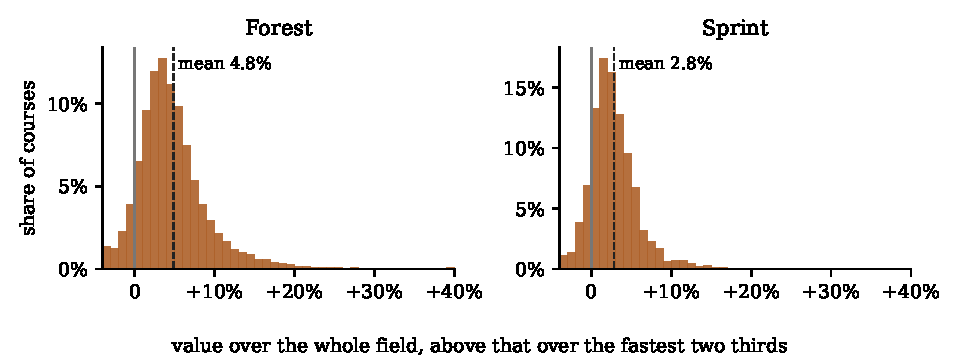
\includegraphics{fig_trunc.pdf}
\caption{For each course, from 2012 to 2026: how far the value measured over the whole field is above that over the fastest two thirds.}\label{fig:trunc}\end{figure}

The share was set in each discipline by a single criterion: the one that best predicts the duels from 2012 to 2024, with no significant loss since July 2025 (figure~\ref{fig:share}).
\begin{itemize}
  \item \textbf{Forest: 90\%.} The whole field gains \NallVsTwoF{} points over the two thirds, and 90\% a further \NnineVsAll{} over the whole field (\NnineVsAllN{} on national races), better in \NnineBetter{} seasons out of 15 and worse in \NnineWorse. The last tenth are the races where runners got badly lost: leaving them out stops a single lost runner from carrying the course value.
  \item \textbf{Sprint: two thirds}, FFCO's rule. Nothing does better over the fifteen seasons; the whole field gives \NallVsTwoS. Mistakes are half as common there as in forest.
  \item \textbf{MTB: 75\%} (\NvttSeventyFive). 85\% does best from 2012 to 2024 (\NvttEightyFive), but loses since July 2025 (\NvttEightyFiveT). \textbf{Ski: 75\%}, as in MTB: it has too few races to be measured.
\end{itemize}

\begin{figure}[h]\centering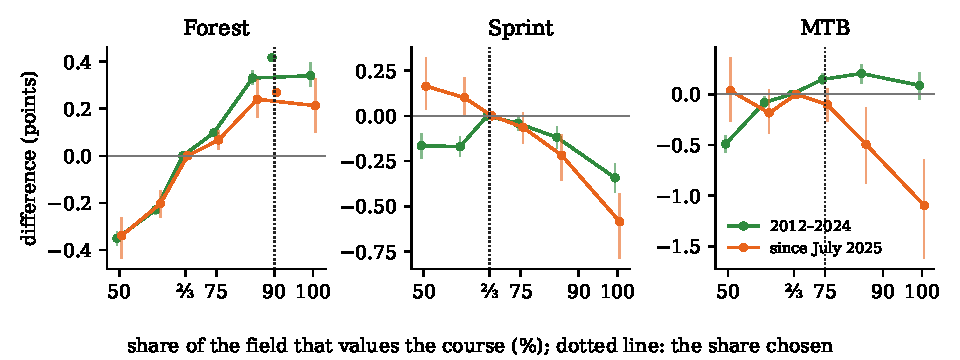
\includegraphics{fig_share.pdf}
\caption{Difference in the share of duels called right compared with the fastest two thirds, in points, by the share of the field that values the course, with the 95\% interval. In forest, the point at 90\% is measured against the whole field.}\label{fig:share}\end{figure}

\paragraph{Juniors' races (19 October 2026).} A junior's \CN{} lags behind their level: a year and a half later, a junior's usual level has risen by 22\% in forest, an adult's by 11\% (the general rise of the scale included). Their races of ten months ago describe a slower runner. A race run in a junior class (M and W up to 20) therefore counts in the mean for $1 - \text{age} / \text{window}$: in full on the race's day, half six months later, hardly at all at the end of the window. It keeps its places; adults' races keep their weight; the rule applies to the usual level, which values the courses, as to the Ozimut index. Each rule's index was read on the day itself, fifteen days before each race.
\begin{itemize}
  \item \textbf{Forest}: \NjunF{} points from 2012 to 2024, better in \NjunFBetter{} seasons of 15, \NjunFT{} since July 2025.
  \item \textbf{Sprint}: \NjunS{} from 2012 to 2024, nothing significant since July 2025 (\NjunST).
  \item \textbf{MTB}: \NjunV{} from 2012 to 2024, \NjunVT{} since July 2025.
\end{itemize}
Ageing every runner's races brings little: at best \NjunAdult{} in forest (the weight halved every six months), and nothing more once the juniors' races fade (\NjunBoth{} with both). An adult's level changes little from one season to the next. A two-year window gives \NjunWin; fading the races in the Ozimut index alone, leaving the usual level as it was, \NjunTop. The price: in forest, juniors are predicted ahead of M/W\,21--34 a little more often than they finish ahead (\NjunBiasBefore{} points before, \NjunBiasAfter{} after); in sprint and MTB, where they were underrated, the gap narrows. A junior's index can now move between two races.

\paragraph{Runners far from their level (18 October 2026).} On a course, a few runners finish far from what their usual level predicts: much faster, often juniors who are improving and whose level was indeed too low (a year later, 17 to 19\% above the other runners of their age), or much slower, after a mistake. 28 rules tried to leave them out of the course value: on one side or both, beyond a threshold or as a fixed share, and to stop juniors from valuing courses. Leaving out the fastest only raises the juniors' courses, so their \CN s, so the value of their next courses: in forest, their courses end up as much as \NoutLoop\% above the adults', and predictions get worse (\NoutFast, \NoutFastFive{} at the 5\% threshold). Leaving out both sides costs in forest (\NoutBothF); in sprint and MTB, together with leaving the juniors out, it gains \NoutXS{} and \NoutXV. Those gains would take two more rules in valuing a course, to correct the same flaw as the fading of the juniors' races: a junior's \CN{} lagging behind their level. The method keeps the course value as it is and treats that lag where it arises, in the index.

\paragraph{The rescaling.} A runner's Ozimut index is made of their best races, so it sits a little above their ordinary races; the following courses are valued with these slightly high levels, and the general level rises by a few tenths of a per cent a month. The factor for a day used to be worked out from a level 18 to 20 months out of date, and the published level overshot the target by 7\% in forest. Carrying the 13-month mean forward at the pace of the rise over the last ten years keeps the factor just as smooth, and brings the published level back close to the target: since 2018, within 2\% on average in forest and MTB and 3\% in sprint, with gaps of 6 to 9\% after the Covid seasons.

\paragraph{Other ideas.} Each idea was recalculated and judged in the same way; none was kept.
\begin{itemize}
  \item \emph{A geometric mean for the course value} (multiplying the products usual level $\times$ time together and taking the root, instead of adding them up): against the Ozimut method, on the same runners, \NgeoVarF{} points of duels in forest and \NgeoVarS{} in sprint. Slightly better in sprint, it was set aside because the ordinary mean can be worked out by hand.
  \item \emph{Making slow times cost more}, by raising the time to a power: this in fact amounted to changing the means of the course and of the \CN; the quadratic mean, online from 7 to 13 October, shook up the rankings without correcting the share of the field.
  \item \emph{A time-to-score rule specific to each course}: worse; with twenty or so runners, the estimate is too uncertain.
  \item \emph{More weight for the races that separate runners better}: no significant difference.
  \item \emph{A score that penalises very large time losses less}: slightly better in forest, clearly worse in sprint.
  \item \emph{The level estimated by a statistical model} that separates the form of the day from mistakes: \NmleS{} points in sprint, \NmleF{} in forest, where making frequent mistakes is a trait of the runner.
  \item \emph{Damping outlying times} (Huber's method) instead of setting the share of the field: about 0.1 points less.
  \item \emph{One course value shared by sprint courses of the same length}, \emph{a score based on the gap to the mean time}, as the IOF does, \emph{a rescaling that reacts to its own effects}: worse, or unstable.
\end{itemize}

\section{Results}

Over the 2012 to 2024 seasons, which were not used for tuning, and on the same runners:
\begin{center}\small
\begin{tabular}{@{}lrrrr@{}}\toprule
 & \multicolumn{2}{c}{Forest} & \multicolumn{2}{c}{Sprint} \\
 & official & Ozimut & official & Ozimut \\ \midrule
duels called right & \NaccFoff\% & \NaccFtop\% & \NaccSoff\% & \NaccStop\% \\
time differences explained & \NrrFoff\% & \NrrFtop\% & \NrrSoff\% & \NrrStop\% \\ \midrule
gain of the Ozimut index in duels, all races & \multicolumn{2}{c}{\NgainF} & \multicolumn{2}{c}{\NgainS} \\
gain of the Ozimut index in duels, national races & \multicolumn{2}{c}{\NgainNF} & \multicolumn{2}{c}{\NgainNS} \\
gain of the Ozimut index in time differences explained & \multicolumn{2}{c}{\NgainRF} & \multicolumn{2}{c}{\NgainRS} \\
seasons in which the gain is significant & \multicolumn{2}{c}{\NwinsF} & \multicolumn{2}{c}{\NwinsS} \\ \bottomrule
\end{tabular}
\end{center}
These figures cover \NcompsF{} forest competitions and \NcompsS{} sprint ones, each course weighted by its number of runners; the gains are in points, with their 95\% interval. Juniors, whom the official \CN{} underrates by \NcalibYoungOff\% in forest compared with M21 and W21 (their courses cause many mistakes), were rated correctly when the whole field valued the course (study of 13 October). Veterans remain overrated by 8 to 9\% by every method, the official one included: the cause is not the way the course is valued.

\section{Conclusion: the simplest of those that predict best}

All the variants tried lie within a few tenths of a point of one another in duels called right, and the best within a few hundredths. At that level, a gain no longer shows in a ranking, but a complicated rule shows in every explanation. The method chosen therefore keeps FFCO's score and ordinary means, and changes only what really matters: the best races kept, filling six places; a share of the field set for each discipline to value the courses (90\% in forest, two thirds in sprint, 75\% in MTB and ski); a continuous rescaling; and juniors' races that count less and less as they age. It gains more than two points of duels over the official \CN, in forest as in sprint.

On the Ozimut site, the official ranking remains the only authoritative reference. The data come from FFCO's national ranking site: a race that is missing, entered wrongly or corrected later may explain a difference. The methods calculated by the site start from the \CN s of 2010, and their first months mostly reflect that starting point.

\end{document}
